\documentclass[tikz,border=5pt]{standalone}
\usepackage{amsmath}
\usepackage{graphicx}
\usetikzlibrary{arrows.meta,positioning,calc}

\definecolor{slategray}{HTML}{374151}
\definecolor{inputblue}{HTML}{2563EB}
\definecolor{inputfill}{HTML}{DCE9F7}
\definecolor{targetgreen}{HTML}{15803D}
\definecolor{targetfill}{HTML}{DCFCE7}
\definecolor{baselinegray}{HTML}{6B7280}
\definecolor{baselinefill}{HTML}{F3F4F6}
\definecolor{resorange}{HTML}{C2410C}
\definecolor{resfill}{HTML}{FFEDD5}
\definecolor{amberdark}{HTML}{B45309}
\definecolor{amberfill}{HTML}{FEF3C7}
\definecolor{evalpurple}{HTML}{7E22CE}
\definecolor{evalfill}{HTML}{F3E8FF}

\begin{document}
\resizebox{\columnwidth}{!}{%
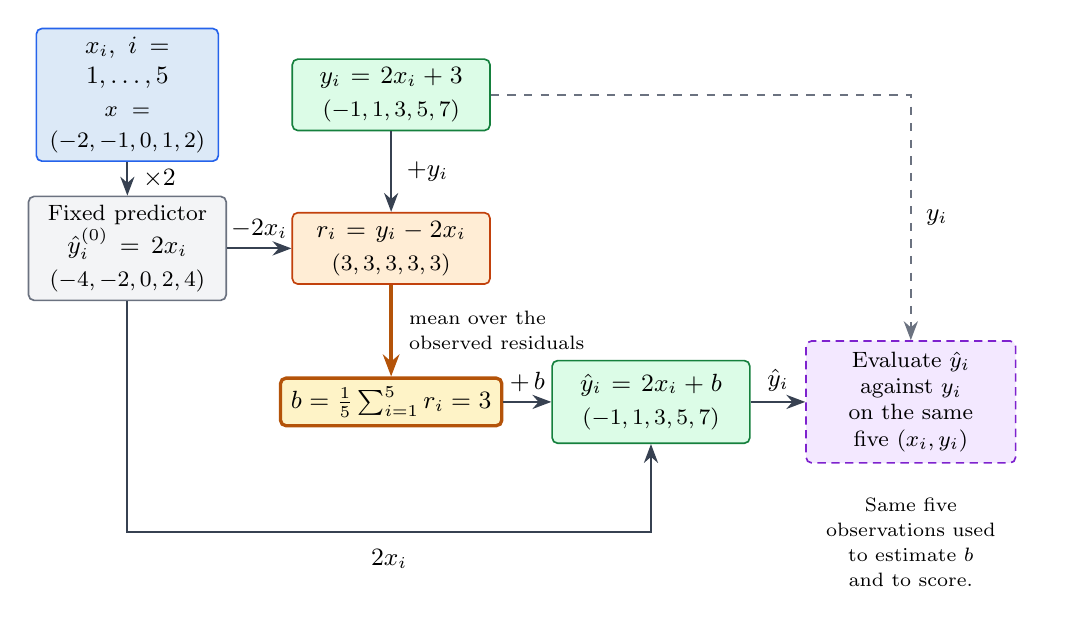
\begin{tikzpicture}[
  font=\small,
  base/.style={
    rounded corners=2pt,
    line width=0.6pt,
    align=center,
    inner sep=3pt
  },
  inputbox/.style={base, draw=inputblue, fill=inputfill, text width=2.1cm},
  targetbox/.style={base, draw=targetgreen, fill=targetfill, text width=2.3cm},
  baselinebox/.style={base, draw=baselinegray, fill=baselinefill, text width=2.3cm},
  residualbox/.style={base, draw=resorange, fill=resfill, text width=2.3cm},
  meanbox/.style={base, draw=amberdark, fill=amberfill, line width=1.2pt,
                  text width=2.6cm},
  corrbox/.style={base, draw=targetgreen, fill=targetfill, text width=2.3cm,
                 minimum height=1.05cm},
  evalbox/.style={base, draw=evalpurple, fill=evalfill, text width=2.45cm,
                  inner ysep=4pt, dash pattern=on 3pt off 2pt,
                  font=\footnotesize, minimum height=1.05cm},
  arr/.style={-{Stealth[length=2.4mm]}, line width=0.7pt, draw=slategray},
  amberarr/.style={-{Stealth[length=2.8mm]}, line width=1.2pt, draw=amberdark},
  grayarr/.style={-{Stealth[length=2.4mm]}, line width=0.7pt,
                  draw=baselinegray, dashed},
  note/.style={font=\fontsize{7.5}{9}\selectfont, align=left}
]

% ------------------------------------------------------------------ nodes
\node[inputbox] (input) at (1.25,5.0)
  {$x_i,\ i=1,\dots,5$\\[1pt]{\footnotesize $x=(-2,-1,0,1,2)$}};

\node[targetbox] (target) at (4.6,5.0)
  {$y_i = 2x_i + 3$\\[1pt]{\footnotesize $(-1,1,3,5,7)$}};

\node[baselinebox] (baseline) at (1.25,3.05)
  {{\footnotesize Fixed predictor}\\[1pt]$\hat{y}_i^{(0)} = 2x_i$\\[1pt]
   {\footnotesize $(-4,-2,0,2,4)$}};

\node[residualbox] (residual) at (4.6,3.05)
  {$r_i = y_i - 2x_i$\\[1pt]{\footnotesize $(3,3,3,3,3)$}};

\node[meanbox] (mean) at (4.6,1.1)
  {$b = \frac{1}{5}\sum_{i=1}^{5} r_i = 3$};

\node[corrbox] (corr) at (7.9,1.1)
  {$\hat{y}_i = 2x_i + b$\\[1pt]{\footnotesize $(-1,1,3,5,7)$}};

\node[evalbox] (eval) at (11.2,1.1)
  {Evaluate $\hat{y}_i$ against $y_i$\\on the same five $(x_i, y_i)$};

% ------------------------------------------------------------------ edges
% input -> baseline
\draw[arr] (input.south) -- (baseline.north)
  node[midway, right=2pt] {$\times 2$};

% target -> residual
\draw[arr] (target.south) -- (residual.north)
  node[midway, right=2pt] {$+y_i$};

% baseline -> residual
\draw[arr] (baseline.east) -- (residual.west)
  node[midway, above] {$-2x_i$};

% residual -> mean (emphasized amber dependency)
\draw[amberarr] (residual.south) -- (mean.north);
\node[note, anchor=west]
  at ([xshift=3pt]$(residual.south)!0.5!(mean.north)$)
  {mean over the\\observed residuals};

% mean -> corrected (additive correction)
\draw[arr] (mean.east) -- (corr.west)
  node[midway, above] {$+\,b$};

% corrected -> evaluation
\draw[arr] (corr.east) -- (eval.west)
  node[midway, above] {$\hat{y}_i$};

% baseline feed: drop, run along lower margin, rise into corrected
\coordinate (feedlevel) at (0,-0.55);
\draw[arr] (baseline.south) -- (baseline.south |- feedlevel)
  -- (corr.south |- feedlevel) -- (corr.south);
\node[font=\small, below=3pt]
  at ($(baseline.south |- feedlevel)!0.5!(corr.south |- feedlevel)$)
  {$2x_i$};

% target -> evaluation (dashed gray elbow, high channel, vertical drop)
\draw[grayarr] (target.east) -| (eval.north);
\node[font=\small, anchor=west]
  at ([xshift=2pt]$(target.east -| eval.north)!0.5!(eval.north)$)
  {$y_i$};

% reuse callout, strictly below the evaluation node
\node[font=\fontsize{7.5}{9}\selectfont, align=center, text width=3.2cm,
      anchor=north] at ([yshift=-9pt]eval.south)
  {\hyphenpenalty=10000 Same five observations used\\to estimate $b$ and to score.};

\end{tikzpicture}%
}
\end{document}